\chapter[Submodular functions]{Submodular functions\raisebox{.3\baselineskip}{\normalsize\footnotemark}}
\footnotetext{Part of this chapter is taken from \href{https://github.com/Halolegend94/uni_social_behavioral_networks/blob/master/chapters/ch03-submodular.tex}{this repo} by \href{https://github.com/Halolegend94}{Cristian Di Pietrantonio}.}\label{sec:submodular-chapter}

In this section we will present a class of functions, called submodular functions, that generate a class of optimization problems that can be solved with the same algorithm (under some other assumptions). To start this topic we first introduce a problem of this class, the Max cover problem.

\section{Max Cover Problem}

\begin{defn}[Max Cover]\label{max-cover}
    Let $X=[n]$ be the ground set, $\mathscr{S}=2^X$, $k\geq1$ be a a parameter of the problem. The Max cover problem consists in finding
    $\max_{\mathscr{C} \subseteq \mathscr{S},\ |\mathscr{C}|=k} f(\mathscr{C})$, where
    \begin{equation}\label{eq:coverage}
        f(\mathscr{C}) = \abs{\bigcup_{S \subset \mathscr{C}} S}
    \end{equation}
    is the \textit{coverage function}.
\end{defn}

In other words, the objective of the max cover problem is to maximize the number of nodes ``covered'' at least one time by a fixed size set of nodes.

\begin{ex}\label{ex:mcp-ex1}
    Let $G$ be the social graph in picture [\ref{fig:mcp-ex1}], and let $k=2$ the number of influencers we want to give our product as gifts, so that they will advertise it in such a way that as many people as possible will know about our product.
    
    \begin{figure}[h!]
        \centering
        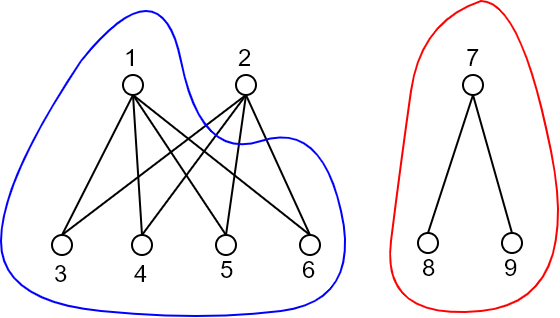
\includegraphics[scale=0.4]{mcp-ex1}
        \caption{An example of max cover on graph $G$.}
        \label{fig:mcp-ex1}
    \end{figure}

    $\mathscr{S} = \{ \{1,3,4,5,6\}, \{2,3,4,5,6\}, \{1,3\}, \{2,3\}, \{1,4\}, \{2,4\}, \{1,5\}, \{2,5\}, \{1,6\}, \{2,6\}, \{7,8,9\}, \{7,8\}, \{7,9\} \}$ is the set of the neighbors of each node. To cover as many users as possible we choose as the best influencers the nodes 1 and 7.\\
    Note that even if node 2 has more friends than node 7, it would cover the same nodes as 1, so it wouldn't be useful.
\end{ex}

Now we present a greedy algorithm that gives an approximation for the max cover problem:
\begin{lstlisting}[caption={The Greedy algorithm to solve the densest subgraph problem},label={lst:mcp-greedy}]
Greedy($\mathscr{S}, k$):
    $\mathscr{S}_0 \gets \emptyset$
    for $i = 1, \ldots, k$:
        let $S_i \in \mathscr{S}$ be a set that maximizes $f \left( \mathscr{C}_{i-1} \cup \{S_i\} \right)$
        $\mathscr{C}_i \gets \mathscr{C}_{i-1} \cup \{S_i\}$
    return $\mathscr{C}_k$
\end{lstlisting}

Note that, at each step, we try all the possible sets $S_i$, and we pick the one that, united to the previous partial solution $\mathscr{C}_{i-1}$, gives the highest value for $f$, maximizing the next partial solution $\mathscr{C}_i$. Another way of seeing this operation is that, at each step, the algorithm removes the nodes already considered into $\mathscr{C}_{i-1}$, before choosing the possible $S_i$s.

\begin{ex}
    Now we can look at example [\ref{ex:mcp-ex1}] with a different prospective:
    
    \begin{figure}[h!]
        \centering
        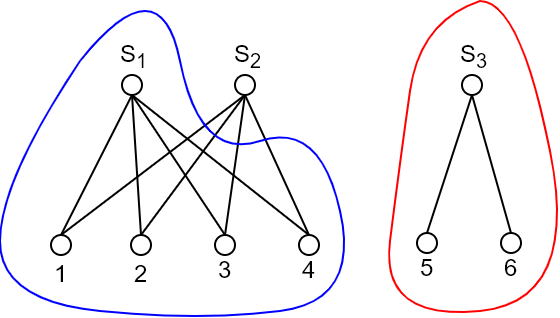
\includegraphics[scale=0.4]{mcp-ex2}
        \caption{An example of application of [\ref{lst:mcp-greedy}].}
        \label{fig:mcp-ex2}
    \end{figure}

    Now the nodes in the upper part of the graph are the names of the sets we are considering, and the other are the nodes they contain, so $S_1 = S_2 = \{1,2,3,4\}$, $S_3 = \{5,6\}$ and $k=2$ as before.
    
    At the beginning we have $\mathscr{C}_0 \gets \emptyset$; then we choose at random between $S_1$ and $S_2$, since they give the same result, so we obtain $\mathscr{C}_1 \gets \{S_1\}$; finally, we consider the two possibilities $\{S_1, S_2\}$ and $\{S_1, S_3\}$, but the first one doesn't give any improvement, so we pick $S_3$ and we obtain $\mathscr{C}_2 \gets \{S_1, S_3\}$, that in this case is the optimal solution.
\end{ex}

\begin{thm}\label{thm:mcp-greedy}
    The algorithm Greedy, described in [\ref{lst:mcp-greedy}], returns a $\left(1-\frac{1}{e}\right)$-approximation for max cover.
\end{thm}
\begin{proof}
    Let's fix an optimal solution $\mathscr{C}^* = \{S_1^*, S_2^*, \ldots, S_k^*\}$ and let's define
    \begin{equation}\label{eq:mcp-dsa}
        \Delta(S|A) := f(A \cup \{S\}) - f(A) = \sum_{i \in X} [i \in S \wedge \nexists T \in A, i \in T],
    \end{equation}
    i.e., the number of new elements that we can cover with $S$ and that weren't covered before adding $S$.
    
    \begin{lem}\label{l:mcp-1}
        \begin{equation}
            \forall\ i \in {0, 1, \ldots, k-1} \quad
            OPT = f(\mathscr{C}^*) \leq f(\mathscr{C}_i) + k \cdot \left( f(\mathscr{C}_{i+1}) - f(\mathscr{C}_i) \right)
        \end{equation}
    \end{lem}
    \begin{proof}
        \begin{flalign*}
            f(\mathscr{C}^*) &\leq f(\mathscr{C}^* \cup \mathscr{C}_i)
            \tag{by monotonicity of $f$}&\\
            &= f(\mathscr{C}_i) + \left( f(\{S_1^*\} \cup \mathscr{C}_i) - f(\mathscr{C}_i) \right)&\\
            &\phantom{\ = f(\mathscr{C}_i)} + \left( f(\{S_1^*, S_2^*\} \cup \mathscr{C}_i ) - f(\{S_1^*\} \cup \mathscr{C}_i) \right)&\\
            &\phantom{\ = f(\mathscr{C}_i)} + \ldots&\\
            &\phantom{\ = f(\mathscr{C}_i)} + \left( f(\{S_1^*, \ldots, S_{k-1}^*\} \cup \mathscr{C}_i ) - f(\{S_1^*, \ldots, S_{k-2}^*\} \cup \mathscr{C}_i) \right)&\\
            &\phantom{\ = f(\mathscr{C}_i)} + \left( f(\mathscr{C}^* \cup \mathscr{C}_i \right) - f(\{S_1^*, \ldots, S_{k-1}^*\} \cup \mathscr{C}_i)&\tag{telescoping series -- see $(*^1)$}\\
            &= f(\mathscr{C}_i) + \sum_{j=1}^{k} \left( f(\{S_1^*, \ldots, S_j^*\} \cup \mathscr{C}_i) - f(\{S_1^*, \ldots, S_{j-1}^*\} \cup \mathscr{C}_i) \right)&\tag{just a more compact way to write the same thing}\\
            &= f(\mathscr{C}_i) + \sum_{j=1}^{k} \Delta (S_j^* \st \{S_1^*, \ldots, S_{j-1}^*\} \cup \mathscr{C}_i)&\tag{by definition of $\Delta$ [\ref{eq:mcp-dsa}]}\\
            &\leq f(\mathscr{C}_i) + \sum_{j=1}^{k} \Delta (S_j^* \st \mathscr{C}_i)&\tag{by diminishing returns -- see $(*^2)$}\\
            &\leq f(\mathscr{C}_i) + \sum_{j=1}^{k} \Delta (S_{i+1} \st \mathscr{C}_i)&\tag{by $(*^3)$}\\
            &\leq f(\mathscr{C}_i) + k \cdot \Delta (S_{i+1} \st \mathscr{C}_i)&\\
            &\leq f(\mathscr{C}_i) + k \cdot \left( f(\mathscr{C}_{i+1}) - f(\mathscr{C}_i) \right)&
        \end{flalign*}
        In the step marked by $(*^1)$, we ``unpack'' the function $f$ as a \textbf{telescoping series}, where each term, except the first and the last, cancels itself with the next one, so that the result doesn't change, but we can rewrite the expression in a more convenient way for our proof (more about telescoping series \href{https://en.wikipedia.org/wiki/Telescoping_series}{on Wikipedia}).\\
        In the step marked by $(*^2)$, we exploit the \textbf{diminishing returns} property of the function $f$ to give an upper bound, that is, if we already have a big number of sets (i.e., $\{S_1^*, \ldots, S_{j-1}^*\} \cup \mathscr{C}_i$), the gain $\Delta$ a new set $S_j^*$ can give us, is less significant then the gain we obtain if we have less sets (i.e., just $\mathscr{C}_i$) (more about diminishing returns \href{https://en.wikipedia.org/wiki/Diminishing_returns}{on Wikipedia}).\\
        The step marked by $(*^3)$ is due to the fact that Greedy maximizes the value of $S$, so, if $S^*$ had been better then $S_{i+1}$, Greedy would have kept $S^*$, instead of picking a new set $S_{i+1}$.
        Furthermore, let's note that in the steps $(*^2)$ and $(*^3)$ we are removing the dependencies on the optimal solution, first on the left and then on the right in the argument of $\Delta$.
    \end{proof}

    With Lemma [\ref{l:mcp-1}] we shown that, at each step of Greedy, the partial solution $\mathscr{C}_i$ gives an upper bound to the optimal solution.\\
    Now we want to prove that the difference between the partial and the optimal solution, bounded by $k \cdot \left( f(\mathscr{C}_{i+1}) - f(\mathscr{C}_i) \right)$, shrinks as the algorithm proceeds with its iterations.
    
    Let's define the difference between the optimal solution and the partial solution at time $i$ as\\
    $\delta_i := f(\mathscr{C}^*) - f(\mathscr{C}_i)$.
    
    \begin{obs}\label{obs:mcp-1}
        $\delta_i - \delta_{i+1} = f(\mathscr{C}^*) - f(\mathscr{C}_i) - \left( f(\mathscr{C}^*) - f(\mathscr{C}_{i+1}) \right) = f(\mathscr{C}_{i+1}) - f(\mathscr{C}_i)$.
    \end{obs}
    
    \begin{lem}\label{l:mcp-2}
        The difference between the optimal solution and the partial solution at time $i$ decreases as $i$ increases:
        \begin{equation}
            \delta_{i+1} \leq \left(1 - \frac{1}{k}\right) \delta_i.
        \end{equation}
    \end{lem}
    \begin{proof}
        \begin{flalign*}
            &f(\mathscr{C}^*) - f(\mathscr{C}_i) \leq k \cdot \left( f(\mathscr{C}_{i+1}) - f(\mathscr{C}_i) \right)&\tag{by lemma [\ref{l:mcp-1}]}\\
            &\implies \delta_i \leq k \cdot \left( f(\mathscr{C}_{i+1}) - f(\mathscr{C}_i) \right)&\\
            &\implies \delta_i \leq k \cdot \left( \delta_i - \delta_{i+1} \right)&\tag{by observation [\ref{obs:mcp-1}]}\\
            &\implies k \cdot \delta_{i+1} \leq k \cdot \delta_i - \delta_i&\\
            &\implies k \cdot \delta_{i+1} \leq (k-1) \cdot \delta_i&\\
            &\implies \delta_{i+1} \leq \left(1 - \frac{1}{k}\right) \delta_i&
        \end{flalign*}
    \end{proof}

    By applying Lemma [\ref{l:mcp-2}], we can finally prove Theorem [\ref{thm:mcp-greedy}]:
    \begin{flalign*}
        &\delta_0 = f(\mathscr{C}^*) - f(\mathscr{C}_0) = f(\mathscr{C}^*)&\\
        &\delta_1 \leq \left( 1 - \frac{1}{k} \right) \cdot \delta_0 = \left( 1 - \frac{1}{k} \right) \cdot f(\mathscr{C}^*)&\\
        &\cdots&\\
        &\delta_i \leq \left( 1 - \frac{1}{k} \right) \cdot \delta_{i-1} = \left( 1 - \frac{1}{k} \right)^i \cdot f(\mathscr{C}^*)&\\
        &\delta_k \leq \left( 1 - \frac{1}{k} \right)^k \cdot f(\mathscr{C}^*)&\\
        &\text{Thus } f(\mathscr{C}^*) - f(\mathscr{C}_k) \leq \left( 1 - \frac{1}{k} \right)^k \cdot f(\mathscr{C}^*)&\\
        &\implies f(\mathscr{C}_k) \geq \left( 1 - \left( 1 - \frac{1}{k} \right)^k \right) \cdot f(\mathscr{C}^*) \geq \left( 1 - \frac{1}{e} \right) \cdot f(\mathscr{C}^*)&\tag{by limit [\ref{eq:limit-1/e}]}
    \end{flalign*}
    Let's note that $f(\mathscr{C}_k)$ is the value returned by Greedy, so the theorem is proved.
\end{proof}

\begin{cor}
    The greedy algorithm [\ref{lst:mcp-greedy}] is optimal, that is, it gives the best possible approximation to the max cover problem.
\end{cor}

\begin{obs}
    The greedy algorithm [\ref{lst:mcp-greedy}] returns a pretty good approximation of the optimal solution even after only half of the $k$ iterations:
    \begin{flalign*}
        &f(\mathscr{C}^*) - f(\mathscr{C}_i) \leq \left( 1 - \frac{1}{k} \right)^i \cdot f(\mathscr{C}^*)&\\
        &\implies f(\mathscr{C}_i) \geq \left( 1 - \left( 1 - \frac{1}{k} \right)^i \right) \cdot f(\mathscr{C}^*)&\\
        &\implies \text{if } i=\frac{k}{2},\ f(\mathscr{C}_i) \geq \left( 1 - e^{-1/2} \right) \cdot f(\mathscr{C}^*)&
    \end{flalign*}
    This means that taking $k/2$ sets instead of $k$ gives us a worse approximation, but not so worse: note that the approximation we obtain using $k$ is $1-\frac{1}{e} = 0.632$, while the approximation obtained using $k/2$ is $1 - e^{-1/2} = 0.393$.
    
    This result can be extraordinarily useful if we don't actually know the value of $k$.
\end{obs}

An other and even more surprising property is the following one:
\begin{obs}
    Already at the first iteration, Greedy gives us a useful approximation of the optimal solution:
    \begin{flalign*}
        &f(\mathscr{C}^*) - f(\mathscr{C}_1) \leq \left( 1 - \frac{1}{k} \right) \cdot f(\mathscr{C}^*)&\\
        &\implies f(\mathscr{C}_1) \geq \frac{1}{k} \cdot f(\mathscr{C}^*)&
    \end{flalign*}
    This strong and rare property is due to the fact that the first set we pick is the most significant one, since it has the biggest cardinality.
\end{obs}


\subsection{Submodular functions}\label{sec:submodular}

Let's take a function $f: 2^{[n]} \to \mathbb{R}$, we can define three classes of functions:
\begin{defn}[Modular function]\label{def:submodular}
    $f$ is modular if, $\forall\ S, T \subseteq [n]$,
    \begin{equation}\label{eq:modular}
        f(S) + f(T) = f(S \cup T) + f(S \cap T).
    \end{equation}
\end{defn}
\begin{defn}[Submodular function]\label{def:modular}
    $f$ is submodular if, $\forall\ S, T \subseteq [n]$,
    \begin{equation}\label{eq:submodular}
        f(S) + f(T) \geq f(S \cup T) + f(S \cap T).
    \end{equation}
\end{defn}
\begin{defn}[Supermodular function]\label{def:supermodular}
    $f$ is supermodular if, $\forall\ S, T \subseteq [n]$,
    \begin{equation}\label{eq:supermodular}
        f(S) + f(T) \leq f(S \cup T) + f(S \cap T).
    \end{equation}
\end{defn}

\begin{ex}[Modular function]
    The cardinality function is modular:
    \begin{itemize}
        \item $f(S)=|S|$ and $f(T)=|T|$,
        \item $f(S \cap T) = |S \cap T|$,
        \item $f(S \cup T) = |S \cap T| + |S \Delta T$,
        \item $f(S) + f(T) = 2 |S \cap T| + |S \Delta T$,
        \item $2 |S \cap T| + |S \Delta T = |S \cap T| + |S \cap T| + |S \Delta T|$.
    \end{itemize}    
\end{ex}

\begin{ex}[Subodular function]
    The coverage function [\ref{eq:coverage}] is submodular:
    \begin{itemize}
        \item let $S=\{\{1,2\}\}$ and $T = \{\{1\}\}$
        \item $f(S)=2$ and $f(T)=1$,
        \item $f(S \cap T) = 0$,
        \item $f(S \cup T) = 2$,
        \item $f(S) + f(T) = 3$,
        \item $3 > 2$.
    \end{itemize}    
\end{ex}

\begin{thm}\label{thm:modular}
    $f(S)$ is modular iff $\exists\ z, w_1, \ldots, w_{|S|}$ such that
    \begin{equation}
        f(S) = z + \sum_{i \in S} w_i.
    \end{equation}
\end{thm}

\subsection{Submodular functions properties}
\begin{lem}[Diminishing return property] \label{lem:dim-return}
    If $f$ is submodular and $S \subseteq T$, $i \notin T$, then
    \[
        \Delta(i|S) \geq \Delta(i | T)
    \]
\end{lem}

\begin{proof}
    Let's take $A = S \cup {i}, B = T$
    \begin{align*}
        f(A) + f(B) &\geq f(A \cup B) + f(A \cap B) \tag{by submodularity}\\
        f(S \cup \{ i\} ) + f(T) &\geq f(T \cup \{ i\}) + f(S) \tag{by definition of A,B} \\
        f(S \cup \{ i \}) - f(S) &\geq f(T \cup \{i\}) - f(T) \\
        \Delta(i|S) &\geq \Delta(i | T) \tag{by definition of $\Delta$ }
    \end{align*}
\end{proof}

\begin{obs}
    The lemma is actually an ``if and only if''; proof of the inverse implication is left as an exercise.
\end{obs}

\begin{obs}
    If $f$ was modular in \cref{lem:dim-return} the equality would hold instead.
\end{obs}

\begin{lem}\label{lem:submodular-power-function}
    if $f_1, f_2, \dots, f_k: 2^x \mapsto \mathcal{R}$ are submodular, and $\alpha_1, \alpha_2 , \dots, \alpha_k \geq 0$ then
    \[
        g(S) \overset{\Delta}{=} \sum_{i=1}^{k} \alpha_i f_i(S)
    \]
    is submodular as well.
\end{lem}

\begin{proof}
    \begin{align*}
        g(S) + g(T) &= \sum_{i=1}^{k} \alpha_i f_i(S) + \sum_{i=1}^{k} \alpha_i f_i(T) = \sum_{i=1}^{k} \alpha_i f_i(S) + \alpha_i f_i(T) \\
        &= \sum_{i=1}^{k} \alpha_i \left( f_i(S) + f_i(T) \right) \geq \sum_{i=1}^{k} \alpha_i \left(f_i (S \cap T) + f_i (S \cup T) \right) \\
        &= \sum_{i=1}^{k} \alpha_i f_i(S \cap T) + \sum_{i=1}^{k} \alpha_i f_i (S \cup T) \\
        &= g(S \cap T) + g(S \cup T)
    \end{align*}
\end{proof}

\begin{obs}
    If one of the $\alpha$s is negative the \cref{lem:submodular-power-function} doesn't hold.
\end{obs}

\subsubsection{One particular submodular function}

\begin{defn}
    Let $ C \subseteq 2^{[n]}, \ w: C \mapsto \mathcal{R}_{\geq 0 }, \ A \subseteq [n] $
    \[
        f_C(A) = \sum_{S \in C}\left( w(S) \cdot \left[ A \cap S \neq \emptyset \right] \right)
    \]
\end{defn}
%
This function looks for all the sets of a class and sums the weights of the ones that intersect the parameter set.
%
\begin{lem} \label{fC-submodular}
    $f_C(A)$ is submodular.
\end{lem}
%
\begin{proof} 
    Fix $A,B \subseteq [n]$; let 
    \begin{align*}
        C_A &= \left\{ S | S \in C \ \land \ S \cap A \neq \emptyset \ \land \ S \cap B = \emptyset \right\} \\
        C_B &= \left\{ S | S \in C \ \land  \ S \cap B \neq \emptyset \ \land \ S \cap A = \emptyset \right\} \\
        C_{\cap} &= \left\{ S | S \in C \ \land \ S \cap A \neq \emptyset \ \land \ S \cap B \neq \emptyset \right\}
    \end{align*}
    \textit{i.e.}, $C_A$ are the sets that intersect $A$ but not $B$, $C_B$ are the sets that intersect $B$ but not $A$ and $C_{\cap}$ are the sets that intersect both $A$ and $B$.
    %
    \begin{obs}
        The conditions are mutually exclusive.
    \end{obs}
    %
    \begin{align}
        f_C(A) &= \sum_{S \in C_A}w(S) + \sum_{s \in C_{\cap}}w(S) \\
        f_C(B) &= \sum_{S \in C_B}w(S) + \sum_{s \in C_{\cap}}w(S) \\
        f_C(A \cup B) &= \sum_{S \in C_A}w(S) + \sum_{S \in C_B}w(S) + \sum_{s \in C_{\cap}}w(S) \\
        f_C(A \cap B) &\leq \sum_{s \in C_{\cap}}w(S) \label{eq:AcapB-leq-sum}\tag{*}
    \end{align}

    \cref{eq:AcapB-leq-sum} is true because of cases like the one in \cref{fig:sets-intersect-empty}; in general in $C_{\cap}$ there may be more sets than in $A \cap B$.

    \begin{figure}[ht]
        \centering
        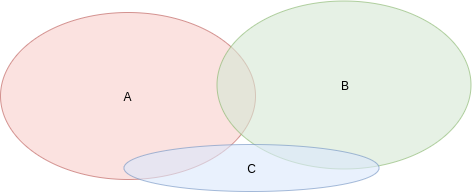
\includegraphics[width=.5\textwidth]{sets-intersect-empty.png}
        \caption{Set C has non-empty intersection with both B and A but does not intersect their intersection.}\label{fig:sets-intersect-empty}
    \end{figure}
    
    So we have that 
    \begin{align}
        f_C(A) + f_C(B) &= \sum_{S \in C_A}w(S) + \sum_{S \in C_B}w(S) + 2 \sum_{S \in C_{\cap}} w(S) \\
                        &= f_C(A \cup B) + \sum_{S \in C_{cap}} w(S) \\
                        &\geq f_C(A \cup B) + f_C(A \cap B) \tag{by inequality \cref{eq:AcapB-leq-sum}}
    \end{align}
\end{proof}

\subsection{KKT model}

KKT stands for Kempe, Kleinsberg and Tardos.
Let's assume we have $k$ gift products to give to $k$ persons for free for marketing reasons; let's assume as well that whenever a person buys the product he keeps it forever.

Moreover, let's assume that time is discrete and that the product spreads over time:
\begin{itemize}
    \item at time $t_0$ the only persons having the product will be the ones that got it for free;
    \item at time $t_i$ for each of the edges incident on the nodes having the product we will be flipping a coin:
    \begin{itemize}
        \item with prob $p$ the product will spread on that edge;
        \item else the edge is lost forever.
    \end{itemize}  
\end{itemize} 

While this point of view is dynamic, there is a static point of view which states the following:
Regardless of which nodes are activated at time 0 what actually happens is that a coin is flipped indipendently for each edge in the graph: 
%
\begin{itemize}
    \item if the coin is $H$ the edge will stay there;
    \item else the edge will be removed (won't be used for spreading the product).
\end{itemize}

Nature will then make its choices, removing some edges. 
By looking at the connected components after nature removes the edges we see that:
%
\begin{itemize}
    \item each connected component containing at least one seed node will be fully conquered;
    \item the others will be forever lost.
\end{itemize}  

If we knew the final components, it would be clear which seed set to choose (we would sort the components in decreasing size and pick one node for each of the first $k$ components); sadly, this is not the case because the set of seed nodes must be chosen a priori.

Suppose that after nature's random choices, A is the set of ``used'' edges, and $C_A$ is the partition of the node set $V$ into connected components with $A$ as the edge set.
Let $R(S)$ be the set of nodes ``conquered'' with seed set $S$; this is clearly a random variable depending on which edges survive.

We can now ask what's the expected cardinality of the reached set $R(S)$ conditioned on the used edges set $A$; we, in fact, would like to maximize this quantity.
%
\begin{align}
    E\left[\abs{R(S)} \big\rvert A\right] = \sum_{T \in C_A}{\left( \abs{T} \cdot \left[ T \cap S \neq \emptyset \right] \right)} \overset{\Delta}{=} f_A(S)
\end{align}

\begin{claim}
    $f_A$ is submodular. 
\end{claim}

\begin{proof}
    See \cref{fC-submodular}.
\end{proof}

Moreover, we can define the expected value as a function of $S$ without conditioning it on a particular $A$ by using the law of total expectation.
\begin{align}
    f(S) = \sum_{A \subseteq E}\left( f_A(S) \cdot Pr\left\{ \text{A is the set of survived edges} \right\} \right) = E\left[ \abs{R(S)} \right]
\end{align}

\begin{claim}
    $f(S)$ is submodular.
\end{claim}

\begin{proof}
    Follows from \cref{lem:submodular-power-function}.
\end{proof}

The problem in optimazing this function is that computing it on a single set takes exponential time, but it can be approximated very well; as an exercise you can try to give the best sampling algorithm to do it.

\subsection{Greedy}

Now we present a greedy algorithm that gives an approximation for $f$:

\begin{lstlisting}[caption={Greedy algorithm},label={lst:fS-greedy}]
$Greedy_{f,\varepsilon}$($k$):
    $S_0 \gets \emptyset$
    for $i = 1, \ldots, k$:
        let $x_i \ be \ s.t. \ \Delta(x_i|S_{i-1}) \geq (1- \varepsilon) \cdot \max_x \Delta(x | S_{i-1})$
        $S_i \gets S_{i-1} \cup \{x_i\}$
    return $S_k$
\end{lstlisting}

\begin{thm}
    If $f$ is monotone, non-negative and submodular GREEDY returns a $(1-e^{-1+\epsilon})$-approximation.
\end{thm}

\begin{proof}
    \begin{flalign*}
            S^{\star} = {x_1^*, x_2^*, \ldots, x_k^*}   \tag{optimal solution}&\\
            \forall i \in  \{0, \ldots, k-1\}&\\
            f(S^*) &\leq f(S^* \cup S_i)    \tag{by monotonicity of $f$}&\\
            &= f(S_i) + \left( f(\{x_1^*\} \cup S_i) - f(S_i) \right)&\\
            &\phantom{\ = f(S_i)} + \left( f(\{x_1^*, x_2^*\} \cup S_i ) - f(\{x_1^*\} \cup S_i) \right)&\\
            &\phantom{\ = f(S_i)} + \ldots&\\
            &\phantom{\ = f(S_i)} + \left( f(\{x_1^*, \ldots, x_{k-1}^*\} \cup S_i ) - f(\{x_1^*, \ldots, x_{k-2}^*\} \cup S_i) \right)&\\
            &\phantom{\ = f(S_i)} + \left( f(S^* \cup S_i \right) - f(\{x_1^*, \ldots, x_{k-1}^*\} \cup S_i)&\tag{telescoping series -- see $(*^1)$}\\
            &= f(S_i) + \Delta(x_1^* | S_i) + \Delta(x_2^* | S_i \cup \{x_1^*\}) + \ldots \Delta(x_k^* | S_i \cup \{x_1^*, \ldots, x_{k-1}^*\})\\
            &= f(S_i) + \sum_{j=1}^{k} \left( \Delta(x_j^* | S_i \cup \{x_1^*, \ldots, x_{j-1}^*\})\right)\\
            &\leq f(S_i) + \sum_{j=1}^{k} \left( \Delta(x_j^* | S_i )\right)&\tag{by diminishing returns -- see $(*^2)$}\\
            &\leq f(S_i) + \sum_{j=1}^{k} \left( \frac{1}{1-\epsilon}\Delta(x_{i+1} | S_i )\right)&\tag{GREEDY}\\
            &= f(S_i) +\frac{k}{1-\epsilon} \Delta(x_{i+1} | S_i )\\
    \end{flalign*}

    where $(*^1)$ and $(*^2)$ are explained in detail in the proof of \cref{l:mcp-1}.
\end{proof}